\vspace{-0.1in}
\section{Improved Application Performance in DDC}
\label{sec:improved}
\vspace{-0.05in}

\vspace{-0.1in}
\subsection{Low latency remote memory}
\vspace{-0.05in}
\rc{
As we have established in the previously section, a DDC requires 100Gbps bandwidth and 3-5us end-to-end latency. 
Current datacenter network usually has 20us network latency, and by our analysis, 5-7us of end-to-end latency is within reach. 
If we enable RDMA inside the datacenter, which takes aways the overhead at OS layer, we can get latency as low as 3-5us. 
We validate this by building a kernel space RDMA block device driver, and use this block device driver as the swap device.
With the RDMA block device driver, the local machine can swap to remote memory instead of swapping to disk.

We implement the block device driver on a machine with Mellanox 4xFDR Infiniband card.
To maintain high throughput, we first use a batch implementation that batches block requests and sends all of them together to the RDMA NIC.
The driver waits for all the request to come back and notify the upper layer.
We test the block device throughput using \textit{dd} with direct IO, and measure the request latency by instrumenting the driver code.
The block device throughput is only 0.8GB/s and the latency is around 4-16us.
We observed that many block requests are actually contiguous in address, so we merge these request in to one large request. 
With request merging, the throughput becomes 2.6GB/s, which is ~3x better than the batch version. 
The performance of the block device driver can be further improved by issuing RDMA requests asynchronously.
We create a data structure to keep track of all the out going requests and notify the upper layer immediately for each completed request.
This improves the throughput to 3.3GB/s which is as high as a local RamFS, and reduces the request latency to 3-4us (Table \ref{tab:rdma_latency}).

\begin{table}[t]
    \centering
    \small
    \begin{tabular}{ccccc}
    \textbf{Min}	& \textbf{Avg}	& \textbf{Median} & \textbf{99.5 Pcntl}	& \textbf{Max}\\
    \hline
    3394 &	3492&	3438&	4549&	12254\\\hline
    \end{tabular}
    \caption{RDMA block device request latency(ns)}
    \label{tab:rdma_latency}
\end{table}

In current non-NUMA architecture, Linux Kernel only launches one \textit{kswapd} to swap out least recently used pages. 
This could be a bottleneck for apps that heavily use remote memory.
We enable the NUMA\_EMU feature in Linux kernel, which partitions the memory into several regions, and each memory region gets its own \textit{kswapd}. 
This improves the throughput of swapping out memory pages.


The RDMA block device driver provides us a simple and efficient way utilize remote memory. 
We setup the block device as swap space and run the \rc{5} applications evaluated in \S \ref{sec:requirements} with lower latency requirements.
\rc{waiting for joao's results}

}
\rc{
\paragraphb{Measuring swap latency}
We measured the software overhead of swapping on a commodity desktop running
Linux 3.13.0. In order to do so, we needed to collect two data points with
minimal modifications to the codebase --- the overall time spent in the page
fault handler on a swap and the time spent actually accessing disk. Although
convenient measurement tools such as \texttt{ftrace} exist, they introduced
unacceptable overhead for our purposes. We also could not arbitrarily introduce
\texttt{printk} calls within the areas we were measuring, since \texttt{printk}
introduces a noticable overhead when measuring on the order of microseconds. In
order to perform the measurement, we took advantage of the fact that the
\texttt{handle\_mm\_fault} function called by the page fault handler (and which
eventually handles swaps) never utilizes the upper 16 bits of its 32 bit return
value, as evidenced by the \texttt{VM\_FAULT\_*} macros in the \texttt{mm.h}
header.

Thus, we wrap both the body of the \texttt{\_\_do\_page\_fault} function and the
call to the \texttt{swapin\_readahead} function (which performs a swap from
disk) in ktime\_get calls.  We then pack the result of the measurement for the
swapin\_readahead function into the upper 16-bits of its caller,
\texttt{do\_swap\_page}, which propagates the value up to
\texttt{\_\_do\_page\_fault}. Once we have completed measuring the body of
\texttt{\_\_do\_page\_fault}, we print both the latency of the whole
\texttt{\_\_do\_page\_fault} routine, as well as the time spent in
\texttt{swapin\_readahead}. We subtract these and average to find that the
software overhead of page fault handler is 2.47 $\mu$s. This
number is a lower-bound on the software overhead of the handler, because we
assume that all of \texttt{swapin\_readahead} is a ``disk access''. 
This is due to the fact that we cannot neatly instrument inside \texttt{swapin\_readahead} in the same manner since it returns a pointer.

Overall, our measurement code introduces a very small number of bitwise
operations (ANDs, ORs, shifts), one integer subtraction, and four calls to
\texttt{ktime\_get} into the handler, which together have a negligible impact on
measurements.
}

\subsection{COST}






\vspace{-0.1in}
\section{Related Work and Discussion}
\label{sec:discussion}
\vspace{-0.05in}

As mentioned earlier, there are many recent and ongoing efforts to prototype disaggregated hardware. We discussed the salient features of these efforts inline throughout this paper and hence we only briefly elaborate on them here. 

Lim \etal~\cite{ddcHwDesign1, ddcHwDesign2} discuss the trend of growing peak compute-to-memory ratio, warning of the ``memory capacity wall'' and prototype a disaggregated memory blade. Their results demonstrate that memory disaggregation is feasible and can even provide a 10x performance improvement in memory constrained environments. As noted earlier, our study focuses on the (for us) worst-case scenario where applications are not memory constrained in the non-disaggregated scenario and hence the potential performance degradation due to disaggregation is high. For the same reason, we did not consider redesigning applications to exploit the plentiful remote memory available in \dis \rc{ other than the brief discussion in \S\ref{sec:improved}}.

Sudan \etal~\cite{ddcHwDesign3} use an ASIC based interconnect fabric to build a virtualized I/O system for better resource sharing. However, these interconnects are designed for their specific context; the authors neither discuss network support for disaggregation more broadly nor consider the possibility of leveraging known datacenter network technologies to enable disaggregation.

Firebox~\cite{firebox} proposes a holistic architecture redesign of datacenter racks to include $1$Tbps silicon phonics links, high-radix switches, remote nonvolatile memory, and System-on-Chips (SoCs). Theia~\cite{theia} proposes a new network topology that interconnects SoCs at high density. Huawei's DC3.0 (NUWA) system uses a proprietary PCIe-based interconnect. R2C2~\cite{r2c2} proposes new topologies, routing and congestion control designs for rack-scale disaggregation.
None of these efforts evaluate network requirements based on existing workloads as we do, nor do they evaluate the effectiveness of existing network designs in supporting disaggregation, or the possibility of disaggregating at scale.

%Overall, we find that related work confirms our prediction that sub-$5\mu$s latencies are feasible in the near future. 

In an early position paper, Han \etal~\cite{hotnets} measure -- as we do -- the impact of remote memory access latency on application-level performance within a single machine. Our work extends this  understanding to a larger set of workloads and concludes with more stringent requirements on latency and bandwidth than Han \etal do, due to our consideration of shark applications. In addition, we use simulation and emulation to study the impact of queueing delay and transport designs which further raises the bar on our target network performance.

%understanding along the new network-oriented design parameters of latency, bandwidth, and transport.Furthermore, our evaluation includes evaluation of additional applications and runs on a cluster of machines ``in the wild,'' measuring realistic scenarios which may have been hidden in a single-machine setting. 

%\paragraphb{Low Latency}
Multiple recent efforts~\cite{farm,mica,herd,ramcloud} aim to reduce the latency in networked applications through techniques that bypass the kernel networking stack, and so forth. %for significant latency improvements with Infiniband RDMA and direct NIC access. 
%Looking forward, CPU-NIC integration, in which the OS kernel and device driver are more directly involved in the low-level operation of the NIC, is on the Simia
Similarly efforts toward NIC integration by CPU architects~\cite{cpu-nic} promise to enable even further latency-saving optimizations. As we note in \S\ref{ssec:rtt}, such efforts are crucial enablers in meeting our latency targets. 










\begin{figure}
  \centering
    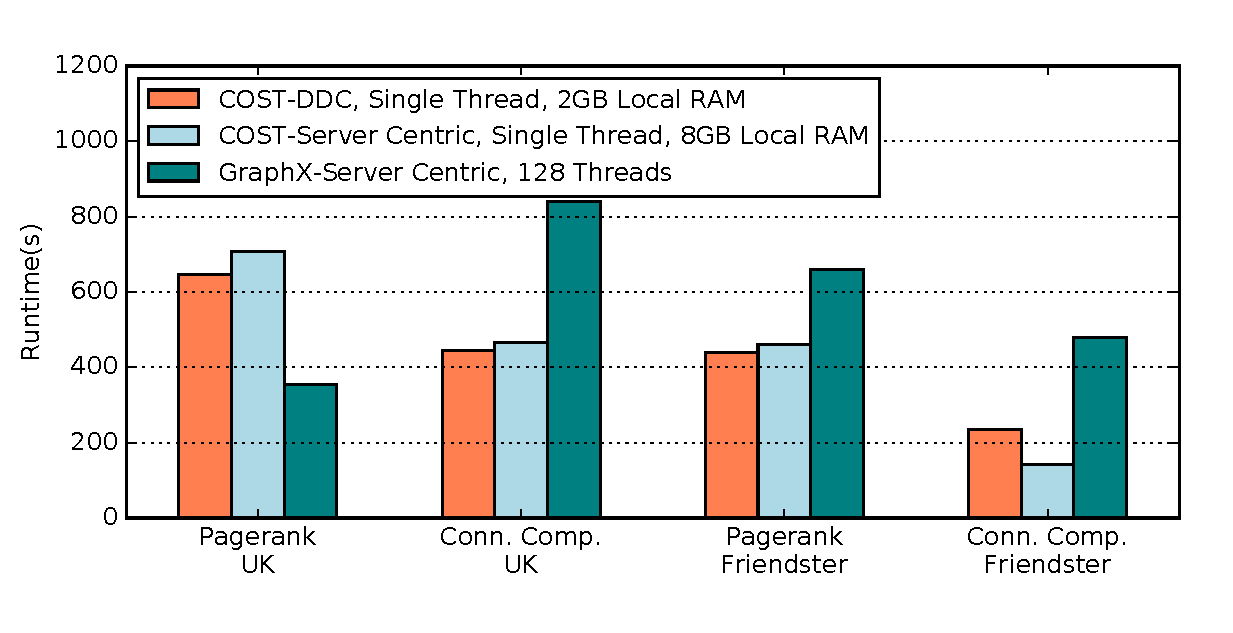
\includegraphics[width = \columnwidth]{img/benefit_uk.eps} 
  \caption{\small{Running COST in a simulated DDC. COST-DDC is 1.48 to 2.05 faster than GraphX-Server Centric except for one case. We use two datasets in our evaluation, UK-2007-05 (105m nodes, 3.7b edges), and Friendster (65m nodes, 1.8b edges)}}
  \label{fig:benefit}
\end{figure}







